	%%  A simple AAU report template.

%  2014-09-13 v. 1.1.0
%  Copyright 2010-2014 by Jesper Kjær Nielsen <jkn@es.aau.dk>
%
%  This is free software: you can redistribute it and/or modify
%  it under the terms of the GNU General Public License as published by
	%  the Free Software Foundation, either version 3 of the License, or
%  (at your option) any later version.
%
%  This is distributed in the hope that it will be useful,
%  but WITHOUT ANY WARRANTY; without even the implied warranty of
%  MERCHANTABILITY or FITNESS FOR A PARTICULAR PURPOSE.  See the
%  GNU General Public License for more details.
%
%  You can find the GNU General Public License at <http://www.gnu.org/licenses/>.
%
%  A simple AAU report template.
%  2014-09-13 v. 1.1.0
%  Copyright 2010-2014 by Jesper Kjær Nielsen <jkn@es.aau.dk>
%
%  This is free software: you can redistribute it and/or modify
%  it under the terms of the GNU General Public License as published by
%  the Free Software Foundation, either version 3 of the License, or
%  (at your option) any later version.
%
%  This is distributed in the hope that it will be useful,
%  but WITHOUT ANY WARRANTY; without even the implied warranty of
%  MERCHANTABILITY or FITNESS FOR A PARTICULAR PURPOSE.  See the
%  GNU General Public License for more details.
%
%  You can find the GNU General Public License at <http://www.gnu.org/licenses/>.
%
\documentclass[11pt,twoside,a4paper,openright]{report}
%%%%%%%%%%%%%%%%%%%%%%%%%%%%%%%%%%%%%%%%%%%%%%%%
% Language, Encoding and Fonts
% http://en.wikibooks.org/wiki/LaTeX/Internationalization
%%%%%%%%%%%%%%%%%%%%%%%%%%%%%%%%%%%%%%%%%%%%%%%%
% Select encoding of your inputs. Depends on
% your operating system and its default input
% encoding. Typically, you should use
%   Linux  : utf8 (most modern Linux distributions)
%            latin1 
%   Windows: ansinew
%            latin1 (works in most cases)
%   Mac    : applemac
% Notice that you can manually change the input
% encoding of your files by selecting "save as"
% an select the desired input encoding. 
\usepackage[utf8]{inputenc}
% Make latex understand and use the typographic
% rules of the language used in the document.
\usepackage[danish,english]{babel}
% Use the vector font Latin Modern which is going
% to be the default font in latex in the future.
\usepackage{lmodern}
% Choose the font encoding
\usepackage[T1]{fontenc}
% For checkmarks: \cmark and crossmarks: \xmark
\usepackage{pifont}
	\newcommand{\cmark}{\ding{51}}%
	\newcommand{\xmark}{\ding{55}}%
%%%%%%%%%%%%%%%%%%%%%%%%%%%%%%%%%%%%%%%%%%%%%%%%
% Graphics and Tables
% http://en.wikibooks.org/wiki/LaTeX/Importing_Graphics
% http://en.wikibooks.org/wiki/LaTeX/Tables
% http://en.wikibooks.org/wiki/LaTeX/Colors
%%%%%%%%%%%%%%%%%%%%%%%%%%%%%%%%%%%%%%%%%%%%%%%%
% load a colour package
\usepackage[table,dvipsnames]{xcolor}
\definecolor{aaublue}{RGB}{33,26,82}% dark blue
\definecolor{lightGrey}{RGB}{240,240,240}% 
% The standard graphics inclusion package
\usepackage{graphicx}
% Load package to convert eps-files to use as figures
\usepackage{epstopdf}

%\usepackage[dvips,final]{graphicx} 
%\usepackage[dvips]{geometry}
\usepackage{color} %include even if images aren’t in color \usepackage{epsfig}
\usepackage{latexsym}
\usepackage{pstricks}

%\usepackage{epsfig}

% Set up how figure and table captions are displayed
\usepackage{caption}
\captionsetup{%
  font=footnotesize,% set font size to footnotesize
  labelfont=bf % bold label (e.g., Figure 3.2) font
}
% For figures
\usepackage{float}
% For subfigures
\usepackage{subcaption}
% Make the standard latex tables look so much better
\usepackage{array,booktabs}
% Enable the use of frames around, e.g., theorems
% The framed package is used in the example environment
\usepackage{framed}
\usepackage{epstopdf}

% Afstand mellem listepunkter og tilføjelse af resume funktion til lister: \begin{enumerate}[resume]
\usepackage{enumitem}
\setlist{itemsep=-2pt}

% Tilføjer mulighed for at lave enkelte sider i landskab.
\usepackage{lscape}
\usepackage{rotating}

\newcounter{listcounter}
%%%%%%%%%%%%%%%%%%%%%%%%%%%%%%%%%%%%%%%%%%%%%%%%
% Mathematics
% http://en.wikibooks.org/wiki/LaTeX/Mathematics
%%%%%%%%%%%%%%%%%%%%%%%%%%%%%%%%%%%%%%%%%%%%%%%%
% Defines new environments such as equation,
% align and split 
\usepackage{amsmath}
% Adds new math symbols
\usepackage{amssymb}
% Use theorems in your document
% The ntheorem package is also used for the example environment
% When using thmmarks, amsmath must be an option as well. Otherwise \eqref doesn't work anymore.
\usepackage[framed,amsmath,thmmarks]{ntheorem}

% Tilføjer \degree symbol
\usepackage{textcomp}
\usepackage{gensymb}

% Fjerner mellemrum efter komma i formler.
%\usepackage{icomma}

% Packages for SI units
\usepackage[binary-units]{siunitx}
% Format SI units as italic in italic texts
\sisetup{detect-all}
\sisetup{per-mode=symbol}


% Argument til amsmath der gør parenteser uden om parenteser pænere ved brug af \right og \left kommandoerne
\delimitershortfall=-1pt

%%%%%%%%%%%%%%%%%%%%%%%%%%%%%%%%%%%%%%%%%%%%%%%%
% Page Layout
% http://en.wikibooks.org/wiki/LaTeX/Page_Layout
%%%%%%%%%%%%%%%%%%%%%%%%%%%%%%%%%%%%%%%%%%%%%%%%
% Change margins, papersize, etc of the document
\usepackage[
  inner=28mm,% left margin on an odd page
  outer=41mm,% right margin on an odd page
  ]{geometry}
% Modify how \chapter, \section, etc. look
% The titlesec package is very configureable
\usepackage[explicit]{titlesec}
%\titleformat*{\section}{\normalfont\Large\bfseries\color{aaublue}}
%\titleformat*{\subsection}{\normalfont\large\bfseries\color{aaublue}}
%\titleformat*{\subsubsection}{\normalfont\normalsize\bfseries\color{aaublue}}
%\titleformat*{\paragraph}{\normalfont\normalsize\bfseries\color{aaublue}}
%\titleformat*{\subparagraph}{\normalfont\normalsize\bfseries\color{aaublue}}
\usepackage{calc}

% Spacing omkring kapiteloverskrift
\titlespacing*{\chapter}{0pt}{40pt}{50pt}

% Overskrift med stort nummer til venstre og titel til højre
%\newlength\chapnumb
%\setlength{\chapnumb}{1.5cm}
%\titleformat{\chapter}[block]
%{\normalfont\bfseries}{}{0pt}
%{\parbox[b]{\chapnumb}{%
	  %\fontsize{2cm}{0}\selectfont\thechapter}%
  %\parbox[b]{\dimexpr\textwidth-\chapnumb\relax}{%
    %\raggedleft%
    %\hfill{\Huge#1}\\
    %\rule{\dimexpr\textwidth-\chapnumb\relax}{.5pt}}}
%\titleformat{name=\chapter,numberless}[block]
%{\normalfont\bfseries}{}{0pt}
	%{\Huge#1}

% Clear empty pages between chapters
\let\origdoublepage\cleardoublepage
\newcommand{\clearemptydoublepage}{%
  \clearpage
  {\pagestyle{empty}\origdoublepage}%
}
\let\cleardoublepage\clearemptydoublepage

% Change the headers and footers
\usepackage{fancyhdr}
\pagestyle{fancy}
\fancyhf{} %delete everything
\renewcommand{\headrulewidth}{0pt} %remove the horizontal line in the header
\fancyhead[RE]{\color{black}\small\nouppercase\leftmark} %even page - chapter title
\fancyhead[LO]{\color{black}\small\nouppercase\rightmark} %uneven page - section title
\fancyhead[LE,RO]{\thepage} %page number on all pages
% Do not stretch the content of a page. Instead,
% insert white space at the bottom of the page
\raggedbottom
% Enable arithmetics with length. Useful when
% typesetting the layout.

\setlength{\headheight}{14pt}

% Raise penalties for bastards
\widowpenalty=10000
\clubpenalty=10000

%%%%%%%%%%%%%%%%%%%%%%%%%%%%%%%%%%%%%%%%%%%%%%%%
% Table of Contents
% http://en.wikibooks.org/wiki/LaTeX/Bibliography_Management
%%%%%%%%%%%%%%%%%%%%%%%%%%%%%%%%%%%%%%%%%%%%%%%%
% Add additional commands for Table of Contents
\usepackage{bookmark}

{\setcounter{tocdepth}{1}}

% Control of space between items in Table of Contents
\usepackage[titles]{tocloft}
\setlength{\cftbeforepartskip}{10pt}
\setlength{\cftbeforechapskip}{4pt}
\setlength{\cftbeforesecskip}{2pt}
%%%%%%%%%%%%%%%%%%%%%%%%%%%%%%%%%%%%%%%%%%%%%%%%
% Bibliography
% http://en.wikibooks.org/wiki/LaTeX/Bibliography_Management
%%%%%%%%%%%%%%%%%%%%%%%%%%%%%%%%%%%%%%%%%%%%%%%%
% Add the \citep{key} command which display a
% reference as [author, year]
\usepackage[square]{natbib}

%%%%%%%%%%%%%%%%%%%%%%%%%%%%%%%%%%%%%%%%%%%%%%%%
% Misc
%%%%%%%%%%%%%%%%%%%%%%%%%%%%%%%%%%%%%%%%%%%%%%%%
% Add bibliography and index to the table of
% contents
\usepackage[nottoc]{tocbibind}
% Add the command \pageref{LastPage} which refers to the
% page number of the last page
\usepackage{lastpage}
\usepackage[
%  disable, %turn off todonotes
  colorinlistoftodos, %enable a coloured square in the list of todos
  textwidth=\marginparwidth, %set the width of the todonotes
  textsize=scriptsize, %size of the text in the todonotes
  ]{todonotes}

% Add command \includepdf to add a whole pdf page to document
\usepackage{pdfpages}


% Add option to easy format directory tree
\usepackage{dirtree}

% String manipulation
\usepackage{xstring,xifthen}

% Tikz package for drawing nice figures
\usepackage{tikz}

% Package for drawing pretty schematics, without leaving LaTex
\usepackage[american currents, american voltages, european resistors, cute inductors,
american ports]{circuitikz}

% Code syntax highlight
\usepackage{listings}
\lstset{breaklines=true,
		breakatwhitespace=true,
		commentstyle=\color{ForestGreen},
		numbers=left,
		numberstyle=\tiny\color{black},
		keywordstyle=\color{blue},
		basicstyle=\footnotesize\ttfamily,
        showstringspaces=false,
		}
\renewcommand{\lstlistingname}{Code Snippet}

%%%%%%%%%%%%%%%%%%%%%%%%%%%%%%%%%%%%%%%%%%%%%%%%
% Table environments
% http://en.wikibooks.org/wiki/LaTeX/Tables
%%%%%%%%%%%%%%%%%%%%%%%%%%%%%%%%%%%%%%%%%%%%%%%%
% Better table environments for stuff like table width specifier
\usepackage{tabularx}
\usepackage{multirow}
\usepackage{longtable}
%%%%%%%%%%%%%%%%%%%%%%%%%%%%%%%%%%%%%%%%%%%%%%%%
% Project info and abstract
% chapters\abstract.tex, chapters\projectinfo.tex
%%%%%%%%%%%%%%%%%%%%%%%%%%%%%%%%%%%%%%%%%%%%%%%%
% Loads project info and abstract for use in
% hypersetup
\newcommand{\projectFaculty}{%
\iflanguage{english}{%
Electronic Engineering and IT%
}{%
Elektronik og IT%
}}

\newcommand{\projectGroup}{%
\iflanguage{english}{%
Group 18gr872%
}{%
Gruppe %
}}

\newcommand{\projectSemester}{%
P8%
}

\newcommand{\projectType}{%
\iflanguage{english}{%
Project Report%
}{%
Projektrapport%
}}

\newcommand{\projectTitle}{%
\iflanguage{english}{%
Low/Mid Frequency Beamforming%
}{%
Low/Mid Frequency Beamforming%
}}

\newcommand{\projectSubtitle}{%
\iflanguage{english}{%
- Subtitle -%
}{%
- Undertitel -%
}}

\newcommand{\projectTheme}{%
\iflanguage{english}{%
Sound technology for the normal hearing%
}{%
Digitale og analoge systemer i samspil med omverdenen%
}}

\newcommand{\projectPeriod}{%
\iflanguage{english}{%
MSc, 8th Semester 2018%
}{%
Efterårssemester 2016%
}}



\newcommand{\projectParticipants}{%
Jonas Buchholdt\\
Christoph Kirsch
}

\newcommand{\projectSupervisors}{%
Christian Sejer Petersen
}

\newcommand{\projectCopies}{8}

\newcommand{\projectCompletion}{
\iflanguage{english}{%
30th may 2018%
}{
30. may 2018%
}}




\newcommand{\projectAbstract}{
This project deals with low/mid frequency directivity control.
The directional characteristics of a single loudspeaker and position of its acoustic center are characterised. An analytical model of the loudspeaker is established to model a beamforming array. After pointing out some properties of the commonly known first order gradient source, a three speaker array is designed. Three speakers are chosen to overcome the disadvantage of the first order gradient speaker not being able to freely control its main lobe direction. To predict the behaviour of the speaker array in a non-free-field environment, a numerical model is set up.  A genetic algorithm is chosen to optimize gain and phase for the individual loudspeakers. A suitable positioning scheme for the speakers is established. Required signal processing parameters are implemented as filters. The measured directional characteristics of the array are compared with the analytical and numerical models and compared with the directional characteristics of a commercial product.

}

\newcommand{\projectSynopsis}{
Synopsis
}

%%%%%%%%%%%%%%%%%%%%%%%%%%%%%%%%%%%%%%%%%%%%%%%%
% Hyperlinks
% http://en.wikibooks.org/wiki/LaTeX/Hyperlinks
%%%%%%%%%%%%%%%%%%%%%%%%%%%%%%%%%%%%%%%%%%%%%%%%
% Enable hyperlinks and insert info into the pdf
% file. Hypperref should be loaded as one of the 
% last packages
\usepackage{hyperref}
\hypersetup{%
	%pdfpagelabels=true,%
	plainpages=false,%
	pdfauthor={\projectGroup, \projectFaculty, \iflanguage{english}{Aalborg University}{Aalborg Universitet}},%
	pdftitle={\projectTitle},%
	pdfsubject={\projectTheme},%
	bookmarksnumbered=true,%
	colorlinks,%
	citecolor=black,%aaublue,%
	filecolor=black,%aaublue,%
	linkcolor=black,%aaublue,% you should probably change this to black before printing
	urlcolor=black,%aaublue,%
	pdfstartview=FitH,%
	bookmarksdepth=2,%
}

% Defines where URLs should break
\def\UrlBreaks{\do\/\do-\do_}
\urlstyle{same}

% Give the possibility to autoformat reference based on distance to the referenced page. Ex. \vpageref{}
\usepackage{varioref}


% Package to warn about missing references.
%\usepackage{refcheck}

% Package to make a glossary of acronyms.
\usepackage{glossaries}
\glstoctrue
\makenoidxglossaries
% Glossaries package
% http://ctan.cs.uu.nl/macros/latex/contrib/glossaries/glossariesbegin.pdf
%
% % % % % % % %
%	Example of glossary entry:
% \newglossaryentry{cabbage}{name={cabbage},description={vegetable with thick green or purple leaves}}
%
%	Example of acronym entry:
% \newacronym{spi}{SPI}{Serial Peripheral Interface}
%


\newacronym{dgps}{DGPS}{Differential \glsentryshort{gps}}


\newacronym{spl}{SPL}{Sound pressure level}
\newacronym{db}{dB}{Decibel}
\newacronym{hz}{Hz}{Hertz}
\newacronym{ft}{FT}{Fourier Transform}
\newacronym{ift}{IFT}{inverse Fourier Transform}
\newacronym{fft}{FFT}{Fast Fourier Transform}
\newacronym{ifft}{IFFT}{inverse Fast Fourier Transform}
\newacronym{ttl}{TTL}{Transistor–transistor logic}
\newacronym{dll}{DLL}{dynamic link library}
\newacronym{udp}{UDP}{User Datagram Protocol}
\newacronym{ip}{IP}{Internet Protocol}
 \newacronym{dut}{DUT}{Device Under Test}
 \newacronym{usb}{USB}{Universal Serial Bus} 
\newacronym{bandk}{B\&K}{Brüel \& Kjær}
\newacronym{mdf}{MDF}{medium-density fibreboard}
\newacronym{rms}{RMS}{Root Mean Square}
\newacronym{fdtd}{FDTD}{Finite-Difference Time-Domain}
\newacronym{sp}{SP}{Signal Processing}
\newacronym{ga}{GA}{Genetic Algorithm}
\newacronym{dc}{DC}{Direct Current}
\newacronym{fir}{FIR}{Finite Impulse Response}
\newacronym{iir}{IIR}{Infinite Impulse Response}
\newacronym{aau}{AAU}{Aalborg University}
\newacronym{bc}{BC}{Bone Conduction}
\newacronym{ac}{AC}{Air Conduction}
\newacronym{hrtf}{HRTF}{Head Related Transfer Function}
\newacronym{bm}{BM}{Basilar Membrane}
\newacronym{best}{BEST}{Balanced Electromagnetic Separation Transducer}







% Package to make semi-bold font.
\usepackage[outline]{contour}
\contourlength{0.1pt}
\contournumber{50}%
\newcommand{\textsb}[1]{\contour{black}{#1}}

% Package for splitting lists or other things up in columns. Ex: \begin{multicols}{2}
\usepackage{multicol}

% Package for rotating a page to landscape orientation. Ex: \begin{landscape}
\usepackage{pdflscape}

% For adding notes to tables
\usepackage{threeparttable}

% For adding smileys ;) I know....
\usepackage{MnSymbol,wasysym}

% For adding algorithms
\usepackage{algorithm}
\usepackage[noend]{algpseudocode}
\makeatletter
\def\BState{\State\hskip-\ALG@thistlm}
\makeatother

\renewcommand*{\glsgroupskip}{\vspace{2mm}}
% ps to PDF


%Highlight
\usepackage{soul}
\usepackage{amsmath}


\usepackage{pdfpages}% Package inclusion and set up of the document

% see, e.g., http://en.wikibooks.org/wiki/LaTeX/Formatting#Hyphenation
% for more information on word hyphenation
\hyphenation{ex-am-ple hy-phen-a-tion short}
\hyphenation{long la-tex}
\hyphenation{AAU-Sat}
\hyphenation{minimum-spændinger}
\hyphenation{ud-vik-lings-poten-tiale}
\hyphenation{pick-up pick-up-pen gui-tar-pick-up gui-tar-pick-up-pen pick-uppens}
\hyphenation{tech-no-lo-gy}
\hyphenation{Hø-re-for-e-ning-en}% Hypenation setup

%  A simple AAU report template.
%  2014-09-13 v. 1.1.0
%  Copyright 2010-2014 by Jesper Kjær Nielsen <jkn@es.aau.dk>
%
%  This is free software: you can redistribute it and/or modify
%  it under the terms of the GNU General Public License as published by
%  the Free Software Foundation, either version 3 of the License, or
%  (at your option) any later version.
%
%  This is distributed in the hope that it will be useful,
%  but WITHOUT ANY WARRANTY; without even the implied warranty of
%  MERCHANTABILITY or FITNESS FOR A PARTICULAR PURPOSE.  See the
%  GNU General Public License for more details.
%
%  You can find the GNU General Public License at <http://www.gnu.org/licenses/>.
%
%
%
% see, e.g., http://en.wikibooks.org/wiki/LaTeX/Customizing_LaTeX#New_commands
% for more information on how to create macros

%%%%%%%%%%%%%%%%%%%%%%%%%%%%%%%%%%%%%%%%%%%%%%%%
% Loads user defined variables
%%%%%%%%%%%%%%%%%%%%%%%%%%%%%%%%%%%%%%%%%%%%%%%%

\newcommand{\noSIunit}{$1$}% Definerer hvad der skal skrives hvis symbolet ikke har nogen enhed.
\newcommand{\obcTransducerAddress}{0xB1}% CAN adresse til tranducer modulet i OBC.

\def\circuitScale{.5}%

%%%%%%%%%%%%%%%%%%%%%%%%%%%%%%%%%%%%%%%%%%%%%%%%
% Macros for the titlepage
%%%%%%%%%%%%%%%%%%%%%%%%%%%%%%%%%%%%%%%%%%%%%%%%
%Creates the aau titlepage
\newcommand{\aautitlepage}[3]{%
  {
    %set up various length
    \ifx\titlepageleftcolumnwidth\undefined
      \newlength{\titlepageleftcolumnwidth}
      \newlength{\titlepagerightcolumnwidth}
    \fi
    \setlength{\titlepageleftcolumnwidth}{0.5\textwidth-\tabcolsep}
    \setlength{\titlepagerightcolumnwidth}{\textwidth-2\tabcolsep-\titlepageleftcolumnwidth}
    %create title page
    \thispagestyle{empty}
    \noindent%
    \begin{tabular}{@{}ll@{}}
      \parbox{\titlepageleftcolumnwidth}{
        \iflanguage{danish}{%
          
\includegraphics[page=1,width=\titlepageleftcolumnwidth]{figures/aau_logo}
        }{%
          
\includegraphics[page=2,width=\titlepageleftcolumnwidth]{figures/aau_logo}
        }
      } &
      \parbox{\titlepagerightcolumnwidth}{\raggedleft\sf\small
        #2
      }\bigskip\\
       #1 &
      \parbox[t]{\titlepagerightcolumnwidth}{%
        \iflanguage{danish}{%
          \textbf{Synopsis:}\smallskip\par
        }{%
          \textbf{Abstract:}\smallskip\par
        }
        \fbox{\parbox{\titlepagerightcolumnwidth-2\fboxsep-2\fboxrule}{%
          #3
        }}
      }\\
    \end{tabular}
    \vfill
    \iflanguage{danish}{%
      \noindent{\footnotesize\emph{Rapportens indhold er frit tilgængeligt, men offentliggørelse (med kildeangivelse) må kun ske efter aftale med forfatterne.}}
    }{%
      \noindent{\footnotesize\emph{The content of this report is freely available, but publication may only be pursued with reference.}}
    }
    \cleardoublepage
  }
}

%Create english project info
\newcommand{\englishprojectinfo}[8]{%
  \parbox[t]{\titlepageleftcolumnwidth}{
    \textbf{Title:}\\ #1\bigskip\par
    \textbf{Theme:}\\ #2\bigskip\par
    \textbf{Project Period:}\\ #3\bigskip\par
    \textbf{Project Group:}\\ #4\bigskip\par
    \textbf{Participants:}\\ #5\bigskip\par
    \textbf{Supervisor:}\\ #6\bigskip\par
    \textbf{Number of Pages:} \pageref{LastPage}\bigskip\par
    \textbf{Date of Completion:}\\ #8
  }
}

%Create danish project info
\newcommand{\danishprojectinfo}[8]{%
  \parbox[t]{\titlepageleftcolumnwidth}{
    \textbf{Titel:}\\ #1\bigskip\par
    \textbf{Tema:}\\ #2\bigskip\par
    \textbf{Projektperiode:}\\ #3\bigskip\par
    \textbf{Projektgruppe:}\\ #4\bigskip\par
    \textbf{Deltagere:}\\ #5\bigskip\par
    \textbf{Vejleder:}\\ #6\bigskip\par
    \textbf{Oplagstal:} #7\bigskip\par
    \textbf{Sidetal:} \pageref{LastPage}\bigskip\par
    \textbf{Afleveringsdato:}\\ #8
  }
}

%%%%%%%%%%%%%%%%%%%%%%%%%%%%%%%%%%%%%%%%%%%%%%%%
% An example environment
%%%%%%%%%%%%%%%%%%%%%%%%%%%%%%%%%%%%%%%%%%%%%%%%
\theoremheaderfont{\normalfont\bfseries}
\theorembodyfont{\normalfont}
\theoremstyle{break}
\def\theoremframecommand{{\color{aaublue!50}\vrule width 5pt \hspace{5pt}}}
\newshadedtheorem{exa}{Example}[chapter]
\newenvironment{example}[1]{%
		\begin{exa}[#1]
}{%
		\end{exa}
}


%%%%%%%%%%%%%%%%%%%%%%%%%%%%%%%%%%%%%%%%%%%%%%%%%
% Exponential function defined as upright e, \exp
%%%%%%%%%%%%%%%%%%%%%%%%%%%%%%%%%%%%%%%%%%%%%%%%%
\renewcommand{\exp}{\text{e}}


%%%%%%%%%%%%%%%%%%%%%%%%%%%%%%%%%%%%%%%%%%%%%%%%%%%
% Command \clearevenpage start chapter on even page
%%%%%%%%%%%%%%%%%%%%%%%%%%%%%%%%%%%%%%%%%%%%%%%%%%%
\makeatletter
\newcommand*{\clearevenpage}{%
  \clearpage
  \if@twoside
    \ifodd\c@page
      \hbox{}%
      \newpage
      \if@twocolumn
        \hbox{}%
        \newpage
      \fi
    \fi
  \fi
}
\makeatother

%%%%%%%%%%%%%%%%%%%%%%%%%%%%%%%%%%%%%%%%%%%%%%%%%%%%%%%
% Command \addunit. Use it to add si units to equations
%%%%%%%%%%%%%%%%%%%%%%%%%%%%%%%%%%%%%%%%%%%%%%%%%%%%%%%
\makeatletter
\providecommand\add@text{}
\newcommand\addunit[1]{%
  \gdef\add@text{\text{[}\ifthenelse{\equal{#1}{}}{\noSIunit}{\si{#1}}\text{]}\gdef\add@text{}}}% 
\renewcommand\tagform@[1]{%
  \maketag@@@{\llap{\add@text\quad}(\ignorespaces#1\unskip\@@italiccorr)}%
}
\makeatother

%%%%%%%%%%%%%%%%%%%%%%%%%%%%%%%%%%%%%%%%%%%%%
% Oversættelser af ord ved brug af \autoref{}
%%%%%%%%%%%%%%%%%%%%%%%%%%%%%%%%%%%%%%%%%%%%%
\addto\extrasdanish{%
  \def\figureautorefname{Figur}%
  \def\subfigureautorefname{Figur}%
  \def\tableautorefname{Tabel}%
  \def\partautorefname{Del}%
  \def\appendixautorefname{Bilag}%
  \def\equationautorefname{Ligning}%
  \def\Itemautorefname{Punkt}%
  \def\chapterautorefname{Kapitel}%
  \def\sectionautorefname{Afsnit}%
  \def\subsectionautorefname{Afsnit}%
  \def\subsubsectionautorefname{Underafsnit}%
  \def\paragraphautorefname{Delafsnit}%
  \def\Hfootnoteautorefname{Fodnote}%
  \def\AMSautorefname{Ligning}%
  \def\theoremautorefname{Sætning}%
  \def\pageautorefname{Side}%
  \def\requirementautorefname{Krav}%
}

\addto\extrasenglish{%
  \def\sectionautorefname{section}%
  \def\subsectionautorefname{section}%
  \def\subsubsectionautorefname{section}%
  \def\requirementautorefname{Requirement}%
  \def\algorithmautorefname{Algorithm}%
}

%%%%%%%%%%%%%%%%%%%%%%%%%%%%%%%%%%%%%%%%%%%%%%%%%%%%%%%%%%%%%%%%%%%%%%
% Tilføjer kommando \fullref{} for både at referere til nummer og navn
%%%%%%%%%%%%%%%%%%%%%%%%%%%%%%%%%%%%%%%%%%%%%%%%%%%%%%%%%%%%%%%%%%%%%%
\renewcommand*{\fullref}[1]{\hyperref[{#1}]{\autoref*{#1} \nameref*{#1}}} % One single link


%%%%%%%%%%%%%%%%%%%%%%%%%%%%%%%%%%%%%%%%%%%%%%%%%%%%%%%%%%%%%%%%%%%%%%
% Tilføjer forkortelser af ord.
%%%%%%%%%%%%%%%%%%%%%%%%%%%%%%%%%%%%%%%%%%%%%%%%%%%%%%%%%%%%%%%%%%%%%%
\newcommand{\AAU}{%
\iflanguage{english}{%
Aalborg University%
}{%
Aalborg Universitet%
}}

\newcommand{\opamp}{%
\iflanguage{english}{%
operational amplifier%
}{%
operationsforstærker%
}}

\newcommand{\hifi}{%
\iflanguage{english}{%
hi-fi amplifier%
}{%
hi-fi-forstærker%
}}

%%%%%%%%%%%%%%%%%%%%%%%%%%%%%%%%%%%%%%%%%%%%%%%%%%%%%%%%%%%%%%%%%%%%%%
% Command \DefVar{VARIBLE_NAME}
% Is used to create a variable.
% Set varible: \VARIBLE_NAME{VALUE}
% Get varible: \getVARIBLE_NAME
%%%%%%%%%%%%%%%%%%%%%%%%%%%%%%%%%%%%%%%%%%%%%%%%%%%%%%%%%%%%%%%%%%%%%%

\makeatletter%
\newcommand{\DefVar}[1]{\@namedef{#1}##1{\global\@namedef{get#1}{##1}}\@nameuse{#1}{}}%
\makeatother%

%%%%%%%%%%%%%%%%%%%%%%%%%%%%%%%%%%%%%%%%%%%%%%%%%%%%%%%%%%%%%%%%%%%%%%
% Requirements environment:
%
% \begin{requirement}
%   \requirement{}
%   \argument{}
%   \fullfilment{}
% \end{requirement}
%%%%%%%%%%%%%%%%%%%%%%%%%%%%%%%%%%%%%%%%%%%%%%%%%%%%%%%%%%%%%%%%%%%%%%

\def\reqPrefixName{??}% Individual prefix for the requirements
\newcounter{reqIDCounter}% Requirement counter for the subsections
\newcounter{requirement}% Absolute requirement counter. Used to trigger label/reference target.

\newlength{\reqBoxWidth}% Create length varible to define width of requirement box
\setlength{\reqBoxWidth}{5cm}% Actual width of requirement box

\newcommand{\reqPrefix}[1]{% Command to define requirement prefix
\ifthenelse{\equal{#1}{}}{\reqPrefixName}{\setcounter{reqIDCounter}{0}\def\reqPrefixName{#1}}%
}

\makeatletter% Define requirementID for references
\newcommand{\reqLabel}{%
\protected@edef\@currentlabel{\reqPrefixName\thereqIDCounter}%
\protected@edef\@currentlabelname{Requirement}%
}\makeatother%

\newenvironment{requirement}%
{\par\vspace{\baselineskip}\noindent\ignorespaces%
\refstepcounter{requirement}%
\stepcounter{reqIDCounter}%
\reqLabel%
\DefVar{requirement}\DefVar{argument}%\DefVar{fullfilment}%
%
\tabularx{1\textwidth}{p{\reqBoxWidth} !{\color{white}{\vrule width 2pt}} X}%
\greyrow \parbox[t]{\reqBoxWidth}{\textsb{Requirement~\reqPrefixName\thereqIDCounter}\\\getrequirement\vskip1mm}%
&%
\parbox[t]{\textwidth-\reqBoxWidth-4\tabcolsep-2pt}{\textsb{Argumentation}\\\getargument\vskip1mm}
%\addlinespace[2pt]%
%\greyrow \multicolumn{2}{l}{\parbox{\textwidth-2\tabcolsep}{\vskip1mm\textsb{Conditions of fulfilment}\\\getfullfilment\vskip1mm}}%
}%
{\endtabularx\par\ignorespacesafterend}


%%%%%%%%%%%%%%%%%%%%%%%%%%%%%%%%%%%%%%%%%%%%%%%%%%%%%%%%%%%%%%%%%%%%%%
% Tilføjer kommando \numnameref{labelnavn}
% Kommandoen tilføjer en reference til et afsnit med både nummer og navn.
%%%%%%%%%%%%%%%%%%%%%%%%%%%%%%%%%%%%%%%%%%%%%%%%%%%%%%%%%%%%%%%%%%%%%%
\newcommand{\numnameref}[1]{%
\hyperref[#1]{\autoref{#1}: \nameref{#1}}%
}

%%%%%%%%%%%%%%%%%%%%%%%%%%%%%%%%%%%%%%%%%%%%%%%%%%%%%%%%%%%%%%%%%%%%%%
% Defines subscript as upright text if it contains more than one character.
% 
%%%%%%%%%%%%%%%%%%%%%%%%%%%%%%%%%%%%%%%%%%%%%%%%%%%%%%%%%%%%%%%%%%%%%%

\catcode`\_=12% Makes underscore an inactive character
\begingroup\lccode`~=`\_% Loads underscore character for redefinition
\lowercase{\endgroup\def~}#1{% Start definition of underscore
\StrLen{#1}[\subscriptstringlen]% Determine length of subscript string
\ifthenelse{\subscriptstringlen=1}% Test if subscript string contain one character
{\sb{#1}}% Prints subscript as italic if only one character is present
{\sb{\mathrm{#1}}}}% Prints subscript as upright text if there are more than one character
\AtBeginDocument{\mathcode`\_=\string"8000 }% Makes underscore active only in math mode



%%%%%%%%%%%%%%%%%%%%%%%%%%%%%%%%%%%%%%%%%%%%%%%%%%%%%%%%%%%%%%%%%%%%%%
% Tilføjer kommando \startexplain, \stopexplain og \explain{}{}
% Bruges til forklaringer af ligninger.
%%%%%%%%%%%%%%%%%%%%%%%%%%%%%%%%%%%%%%%%%%%%%%%%%%%%%%%%%%%%%%%%%%%%%%
\newcounter{firstexplain}% Holder styr på om det er den første symbolforklaring

\def\startexplain{%
	\setcounter{firstexplain}{1}%
	{\noindent}%
	{\par\noindent}
	\begin{tabular}{@{}p{.06\columnwidth}p{.76\columnwidth}@{\hskip.04\columnwidth}p{.02\columnwidth}@{}}}%
\def\stopexplain{\end{tabular}\\[10pt]}%

\newcommand{\explain}[2]{%
	\ifthenelse{\thefirstexplain=1}{%
	Where:\\
	&#1&[\ifthenelse{\equal{#2}{}}{\noSIunit}{#2}]\\\setcounter{firstexplain}{0}
	}{%
	&#1&[\ifthenelse{\equal{#2}{}}{\noSIunit}{#2}]\\%
	}%
}%

%%%%%%%%%%%%%%%%%%%%%%%%%%%%%%%%%%%%%%%%%%%%%%%%%%%%%%%%%%%%%%%%%%%%%%
% Tilføjer kommando \startexplain, \stopexplain og \explain{}{}
% Bruges til forklaringer af ligninger.
%%%%%%%%%%%%%%%%%%%%%%%%%%%%%%%%%%%%%%%%%%%%%%%%%%%%%%%%%%%%%%%%%%%%%%





%%%%%%%%%%%%%%%%%%%%%%%%%%%%%%%%%%%%%%%%%%%%%%%%%%%%%%%%%%%%%%%%%%%%%%
% Tilføjer kommando \hyph
% Bruges til bindestreger i ord så de stadig kan deles korrekt af Latex.
%%%%%%%%%%%%%%%%%%%%%%%%%%%%%%%%%%%%%%%%%%%%%%%%%%%%%%%%%%%%%%%%%%%%%%
\def\hyph{-\penalty0\hskip0pt\relax}


%%%%%%%%%%%%%%%%%%%%%%%%%%%%%%%%%%%%%%%%%%%%%%%%%%%%%%%%%%%%%%%%%%%%%%
% Tilføjer kommando \hex og \bin
% Bruges til at skrive hexidecimal og binære tal.
%%%%%%%%%%%%%%%%%%%%%%%%%%%%%%%%%%%%%%%%%%%%%%%%%%%%%%%%%%%%%%%%%%%%%%
\newcommand{\hex}[1]{%
	\texttt{#1$_{16}$}
}%

\newcommand{\bin}[1]{%
	\texttt{#1$_{2}$}
}%


\newcommand{\greyrow}{%
	\rowcolor{lightGrey}
}%


%%%%%%%%%%%%%%%%%%%%%%%%%%%%%%%%%%%%%%%%%%%%%%%%%%%%%%%%%%%%%%%%%%%%%%
% Tilføjer kommando \citeref
% Bruges til at referere til egen rapport/bilag.
%%%%%%%%%%%%%%%%%%%%%%%%%%%%%%%%%%%%%%%%%%%%%%%%%%%%%%%%%%%%%%%%%%%%%%
\newcommand{\citeref}[1]{%
	[\autoref{#1}]%
}%


%%%%%%%%%%%%%%%%%%%%%%%%%%%%%%%%%%%%%%%%%%%%%%%%%%%%%%%%%%%%%%%%%%%%%%
% Tilføjer kommando \rot{}
% Bruges fx til at rotere kollonneoverskrifter i en tabel.
%%%%%%%%%%%%%%%%%%%%%%%%%%%%%%%%%%%%%%%%%%%%%%%%%%%%%%%%%%%%%%%%%%%%%%
\newcommand*\rot{\rotatebox{60}}


%%%%%%%%%%%%%%%%%%%%%%%%%%%%%%%%%%%%%%%%%%%%%%%%%%%%%%%%%%%%%%%%%%%%%%
% Tilføjer kommando \file{}
% Bruges til at indsætte et filnavn i teksten.
%%%%%%%%%%%%%%%%%%%%%%%%%%%%%%%%%%%%%%%%%%%%%%%%%%%%%%%%%%%%%%%%%%%%%%
\newcommand{\file}[1]{\texttt{#1}}

\definecolor{javared}{rgb}{0.6,0,0} % for strings
\definecolor{javagreen}{rgb}{0.25,0.5,0.35} % comments
\definecolor{javapurple}{rgb}{0.5,0,0.35} % keywords
\definecolor{javadocblue}{rgb}{0.25,0.35,0.75} % javadoc
\definecolor{gray}{rgb}{0.4,0.4,0.4}
\definecolor{darkblue}{rgb}{0.0,0.0,0.6}
\definecolor{cyan}{rgb}{0.0,0.6,0.6}
\definecolor{lightblue}{rgb}{0.0,0.3,0.7}
\definecolor{orange}{rgb}{0.8,0.3,0.0}
\definecolor{matlabstring}{rgb}{.627,.126,.941}


%Hvordan XML kode skal se ud
\lstdefinestyle{customXML}{
  belowcaptionskip=1\baselineskip,
  breaklines=true,
  frame=L,
  xleftmargin=\parindent,
  language=XML,
  showstringspaces=false,
  basicstyle=\footnotesize\ttfamily,
  morestring=[b]",
  morestring=[s]{>}{<},
  morecomment=[s]{<?}{?>},
  stringstyle=\color{black},
  identifierstyle=\color{darkblue},
  keywordstyle=\color{cyan},
  morekeywords={xmlns,version,type},
 commentstyle=\color{gray}\upshape,
}


%Hvordan java kode skal se ud
\lstdefinestyle{customjava}{
  belowcaptionskip=1\baselineskip,
  breaklines=true,
  frame=L,
  xleftmargin=\parindent,
  language=java,
  showstringspaces=false,
  basicstyle=\footnotesize\ttfamily,
  keywordstyle=\color{javapurple}\bfseries,
stringstyle=\color{javared},
commentstyle=\color{javagreen},
morecomment=[s][\color{javadocblue}]{/**}{*/},
}

%Hvordan C kode skal se ud
\lstdefinestyle{customc}{
  belowcaptionskip=1\baselineskip,
  breaklines=true,
  frame=L,
  xleftmargin=\parindent,
  language=C,
  showstringspaces=false,
  basicstyle=\footnotesize\ttfamily,
  keywordstyle=\bfseries\color{green!40!black},
  commentstyle=\itshape\color{gray},
  identifierstyle=\color{blue},
  stringstyle=\color{orange},
}

%Hvordan ASM kode skal se ud
\lstdefinestyle{customassembly}{
  belowcaptionskip=1\baselineskip,
  breaklines=true,
  frame=L,
  xleftmargin=\parindent,
  %language=assembly,
  showstringspaces=false,
  basicstyle=\footnotesize\ttfamily,
  keywordstyle=\bfseries\color{green!40!black},
%where there is a space  
  numbers=left,%
  numberstyle={\tiny \color{black}},% size of the numbers
  numbersep=9pt, % this defines how far the numbers are from the text
  commentstyle=\itshape\color{javagreen},
  %assembly structure
  emph=[1]{equ,text,data,word,set},emphstyle=[1]\color{matlabstring}, 
  %commands
  emph=[2]{MOV,mov,BTST,BCC,NOP,RET},emphstyle=[2]\color{gray}, 
  %label
  emph=[3]{in,recieve_flag,out,transmit_flag,buffer,positive,negative,final,case_one,case_two},emphstyle=[3]\color{blue},
  identifierstyle=\color{black},
  stringstyle=\color{blue},
    comment=[l];,                              % comments
}

%Hvordan Matlab kode skal se ud
\lstdefinestyle{custommatlab}{
basicstyle=\footnotesize\ttfamily,
    breaklines=true,%
    morekeywords={matlab2tikz},
    keywordstyle=\color{blue},
    %morekeywords=[2]{1}, 
    keywordstyle=[2]{\color{black}},
    identifierstyle=\color{black},
    morestring=[m]', % defines that strings are enclosed in double quotes
    stringstyle=\color{matlabstring},
    showstringspaces=false,%without this there will be a symbol in the places where there is a space
    numbers=left,%
    numberstyle={\tiny \color{black}},% size of the numbers
    numbersep=9pt, % this defines how far the numbers are from the text
    emph=[1]{if,for,end,break,while,else,function},emphstyle=[1]\color{blue}, %some words to emphasise
    emph=[2]{all,on},emphstyle=[2]\color{matlabstring}, 
% matlat languate definition
  comment=[l]\%,                              % comments
  morecomment=[l]...,                         % comments
  morecomment=[s]{\%\{}{\%\}},                % block comments
  commentstyle=\color{Green},
}

%Hvordan VHDL kode skal se ud
\lstdefinestyle{customVHDL}{
  belowcaptionskip=1\baselineskip,
  breaklines=true,
  frame=L,
  xleftmargin=\parindent,
  language=VHDL,
  showstringspaces=false,
  basicstyle=\footnotesize\ttfamily,
  keywordstyle=\bfseries\color{blue!100!black!80},
  commentstyle=\itshape\color{green!90!black!90},
  identifierstyle=\color{black},
  stringstyle=\color{orange},
}

%Hvordan PHP kode skal se ud
\lstdefinestyle{customPHP}{
  belowcaptionskip=1\baselineskip,
  breaklines=true,
  frame=L,
  xleftmargin=\parindent,
  language=PHP,
  showstringspaces=false,
  basicstyle=\footnotesize\ttfamily,
 keywordstyle    = \color{blue},
  stringstyle     = \color{gray},
  identifierstyle = \color{lightblue},
  commentstyle    = \color{green},
  emph            =[1]{php},
  emphstyle       =[1]\color{black},
}
%Commando til at indsætte kode i latex
\newcommand{\includeCode}[7]{\lstinputlisting[caption=#5 | #1, style=custom#2, numbers=left, firstnumber=#3, firstline=#3, lastline=#4, label=#6]{#7#1}}

%Caption navn foran nummeret i kode
\renewcommand{\lstlistingname}{Code snippet}
\def\lstlistingautorefname{Code snippet}


\makeatletter
%\newcommand*{\getlength}[1]{\strip@pt#1}
% Or rounded back to `mm` (there will be some rounding errors!)
\newcommand*{\getlength}[1]{\strip@pt\dimexpr0.35146\dimexpr#1\relax\relax}
%
\makeatother% Macros

\begin{document}

\selectlanguage{english}

\pagestyle{empty}



%frontmatter
% Indholdsfortegnelse over kommentarer.
% HUSK AT SLETTE INDEN AFLEVERING! -->
%\pagenumbering{alph}
%\pdfbookmark[0]{Todoliste}{label:todos}
%\listoftodos[Notes]
%\cleardoublepage
% <-- HUSK AT SLETTE INDEN AFLEVERING!

 %disable headers and footers
\pagenumbering{roman} %use roman page numbering in the frontmatter

%\pdfbookmark[0]{Forside}{label:forside}%
%\includepdf[fitpaper]{chapters/frontpage.pdf}
%  A simple AAU report template.
%  2014-09-13 v. 1.1.0
%  Copyright 2010-2014 by Jesper Kjær Nielsen <jkn@es.aau.dk>
%
%  This is free software: you can redistribute it and/or modify
%  it under the terms of the GNU General Public License as published by
%  the Free Software Foundation, either version 3 of the License, or
%  (at your option) any later version.
%
%  This is distributed in the hope that it will be useful,
%  but WITHOUT ANY WARRANTY; without even the implied warranty of
%  MERCHANTABILITY or FITNESS FOR A PARTICULAR PURPOSE.  See the
%  GNU General Public License for more details.
%
%  You can find the GNU General Public License at <http://www.gnu.org/licenses/>.
%
\iflanguage{english}
{\pdfbookmark[0]{Frontpage}{label:frontpage}}%
{\pdfbookmark[0]{Forside}{label:forside}}%

\begin{titlepage}
  \addtolength{\hoffset}{0.5\evensidemargin-0.5\oddsidemargin} %set equal margins on the frontpage - remove this line if you want default margins
  \noindent%
  \begin{tabular}{@{}p{\textwidth}@{}}
    \toprule[2pt]
    \midrule
    \vspace{0.2cm}
    \begin{center}
    \huge{\textbf{
      \projectTitle% You can change the title in projectinfo.tex
    }}
    \end{center}
%    \begin{center}
%      \Large{
%        \projectSubtitle% insert your subtitle here
%      }
%    \end{center}
    \vspace{0.2cm}\\
    \midrule
    \toprule[2pt]
  \end{tabular}
  \vspace{4 cm}
  \begin{center}
    {\large
      \projectType%Insert document type (e.g., Project Report)
    }\\
    \vspace{0.2cm}
    {\Large
      \projectGroup%Insert your group name or real names here 
    }
  \end{center}
  \vfill
  \begin{center}
  \iflanguage{english}{Aalborg University}{Aalborg Universitet}\\
  \projectFaculty
  \end{center}
\end{titlepage}
\clearpage

\thispagestyle{empty}
{\small
\strut\vfill % push the content to the bottom of the page
\noindent Copyright \copyright{} \projectGroup{}, \projectFaculty{} \projectSemester{}, \AAU{} \the\year\par
\vspace{0.2cm}
\noindent This report is compiled in \LaTeX. Additionally Mathworks MATLAB\textsuperscript{\textregistered}, Inkscape, and Xfig are used to draw figures and charts.
}
\clearpage

{\iflanguage{english}{
\pdfbookmark[0]{Title Page}{label:titlepage_en}
\aautitlepage{%
  \englishprojectinfo{
    \projectTitle %title 
  }{%
    \projectTheme %theme
  }{%
    \projectPeriod %project period
  }{%
    \projectGroup % project group
  }{%
    \projectParticipants %list of group members
  }{%
    \projectSupervisors %list of supervisors
  }{%
    \projectCopies % number of printed copies
  }{%
    \projectCompletion % date of completion
  }%
}{%department and address
  \textbf{\projectFaculty}\\
  Aalborg University\\
  \href{http://www.aau.dk}{http://www.aau.dk}\\
}{% the abstract
  \projectAbstract
}}
{
\pdfbookmark[0]{Titelblad}{label:titlepage_da}

\aautitlepage{%
  \danishprojectinfo{
    \projectTitle  %title 
  }{%
    \projectTheme %theme
  }{%
    \projectPeriod %project period
  }{%
    \projectGroup % project group
  }{%
    \projectParticipants %list of group members
  }{%
    \projectSupervisors %list of supervisors
  }{%
    \projectCopies % number of printed copies
  }{%
    \projectCompletion % date of completion
  }%
}{%department and address
  \textbf{\projectFaculty}\\
  Aalborg Universitet\\
  \href{http://www.aau.dk}{http://www.aau.dk}\\
}{% the abstract
 \projectSynopsis
}}}


\cleardoublepage
\pagestyle{fancy} % Enable headers and footers again
\iflanguage{english}{
\chapter*{Preface\markboth{Preface}{Preface}}\label{ch:preface}%
\addcontentsline{toc}{chapter}{Preface}%
}{%
\chapter*{Forord\markboth{Forord}{Forord}}\label{ch:forord}%
\addcontentsline{toc}{chapter}{Forord}%
}
This report is composed by group 18gr975 during the 9th semester of \projectFaculty{} at \AAU{}. The general purpose of the report is ?? \textit{\projectTheme}. 

For citations, the report employs the Harvard method. If citations are not present by figures or tables, these have been made by the authors of the report. Units are indicated according to the SI standard.


\vspace{\baselineskip}\hfill \AAU, \today
\vfill\noindent
\begin{center}
\begin{minipage}[b]{0.45\textwidth}
 \centering
  \textit{}\\
 {}
\end{minipage}
\hspace{0.3cm}
\begin{minipage}[b]{0.45\textwidth}
 \centering
  \textit{}\\
 {}
\end{minipage}
\end{center}
\vspace{1\baselineskip}
\begin{center}
\begin{minipage}[b]{0.45\textwidth}
 \centering
  \textit{Jonas Buchholdt}\\
 {\footnotesize <Jbuchh13@student.aau.dk>}
\end{minipage}
\hspace{0.3cm}
\begin{minipage}[b]{0.45\textwidth}
 \centering
  \textit{Christoph Kirsch}\\
 {\footnotesize <Ckirsc17@student.aau.dk>}
\end{minipage}
\vfill\noindent
\begin{minipage}[b]{0.45\textwidth}
 \centering
  \textit{Jorge Bravo}\\
 {\footnotesize <Jbravo12@student.aau.dk>}
\end{minipage}
\end{center}


%\input{chapters/laesevejledning/_laesevejledning}


\begingroup % Let ToC start on even page.
  \let\cleardoublepage\clearevenpage
	\cleardoublepage
	\iflanguage{english}{\pdfbookmark[0]{Contents}{label:contents}}{\pdfbookmark[0]{Indhold}{label:indhold}}
 \tableofcontents
\endgroup

\cleardoublepage

\printnoidxglossaries
% Mainmatter
\pagenumbering{arabic} % Use arabic page numbering in the mainmatter

\glsresetall
 \graphicspath{{figures/analysing/}}
\chapter{Introduction}\label{ch:intro}

The directivity of sound sources is an issue that has an impact on many situations of our daily life, e.g. at live music venues. Voluntary listeners, namely the audience, enjoy comparatively high sound pressure levels when gathering around the stage. Involuntary listeners, generally neighbours, tend to perceive the sound emitted by the stage as a disturbing noise. The extent of this problem may be minimized with directivity control of the sound sources. The concept of directivity control involves more sound energy being emitted towards voluntary listeners and less towards involuntary listeners. 

There are several effects that make directivity control difficult in a certain frequency range. Commonly used loudspeaker contraptions for low/mid frequency playback tend to act like omnidirectional sound sources \citep[p. 1391 f.]{crocker98}.  The dampening of sound as it progresses in air has significantly less influence towards the lower frequencies of the human hearing range than it has towards the higher frequencies \citep[p. 240]{moeser2009}. Additionally, because of the way most houses are built, low frequency sound penetrates through walls and windows to a greater extent than high frequency sound \citep[p. 240 ff.]{moeser2009}. All of these effects lead to neighbours primarily being disturbed by low frequency sound from nearby live music venues.\\

This project aim is directivity control of sound in a frequency range of \SIrange{60}{300}{\hertz}. The lower frequency limit is accounted to practical difficulties producing and measuring sound in the lowest part of the human hearing range. Loudspeakers tend to grow in size, making them difficult to handle and making the speaker cabinets a larger influence on the sound field for higher frequencies. Anechoic environments for frequencies below \SI{60}{\hertz} are very rare, introducing the need to measure outside. With measuring outside a whole range of problems is introduced, like finding a suitable site, having to transport all equipment to that site and being highly sensitive to wind and precipitation. Opposed to that, at \SI{60}{\hertz} and above, measurements under free field conditions can be conducted in the large anechoic chamber of \gls{aau}. Because the beamforming is based on the loudspeakers acting as omnidirectional sound sources (see \autoref{ch:directional}), there is no reason at first glance, why the principles described in this report cannot be utilized for frequencies lower than the target range of the project.\\
The upper frequency limit has been chosen for two reasons. Firstly, the loudspeakers utilized in this project with rising frequency increasingly aberrate from the approximation of an omnidirectional source (see \autoref{sec:beamwidth}). This makes the low frequency model of the loudspeakers as omnidirectional sources less applicable to the actual behaviour of the loudspeakers. With a speed of sound of $c=\SI{343}{\meter\per\second}$, the wavelength at \SI{300}{\hertz} is approx. $\lambda=\SI{1.14}{\meter}$. This makes frequencies above \SI{300}{\hertz} feasible for ``classical'' directivity control approaches, based on horns, which have to have a certain size in relation to the wavelength in order to work \citep{Borwick2012}[p. 35 ff.]. These might not be a practical solution for living room setups, but at the problematic area of public address systems the size is feasible.\\

An established technique for directivity control at low frequencies involves groups of two to four subwoofers placed close to eachother and being pointed in opposite directions. The signal of one of subwoofers is then manipulated in order to create a cardiod radiation pattern \citep{KS28}. This technique is further explained in \autoref{sec:first_order_speaker}.\\
A recent commercial product, the D\&B SL-series, claims to be able to achieve cardiod directivity in a comparatively compact low/mid line array unit containing four drivers. Two of the drivers are pointing towards the front of the module, and the other two are in the sides of the cabinet \citep{SL_GSL}. This inspired the authors of this report to establish another approach on low/mid frequency beamforming. Using three loudspeakers placed in a triangular configuration, it is expected to be possible to form a loudspeaker array that can be set up to have supercardiod radiation characteristics. This might allow for a narrower main lobe as well as making it possible to adjust the mainlobe in relation to the array into any direction by changing the \gls{sp}-parameters on the individual channels of the speakers.






%The difference in the perception of the sound is visualised in \autoref{fig:Problem}.
%
%
%\begin{figure}[htbp]
%	\centering
%	\includegraphics[width=1\textwidth]{change_later.png}
%	\caption{Normalized \gls{spl} in colour, red is high \gls{spl} where blue is low \gls{spl}}
%		\label{fig:Problem}
%\end{figure}
%
%%\autoref{fig:Problem} shows the total sound pressure level \gls{spl} in \gls{db} from \SI{20}{\hertz} to \SI{20}{\kilo\hertz} for the voluntary listeners and the non-voluntary listeners during a concert.
%\autoref{fig:Problem} shows a qualitative drawing of a near-ideal sound pressure distribution in the vicinity of a stage during a concert. The high-\gls{spl}areas are highlighted by red color, and is the area where the voluntary listeners condense. This area is define as the \textbf{participants' area} The non-voluntary listeners are located in the area around the participants' area, that we define as \textbf{the neighbourhood}. 
%
%While a \gls{spl} distribution as depicted in \autoref{fig:Problem} is easier to achieve the higher the frequency gets, towards low frequencies the \gls{spl}distribution might look more like depicted in autoref(fig:problem2).
%
%
%
%The directivity control of mid- and high frequency has a known solution which has been applied for many years. In general, horns are used, which are designed for a particular radiation pattern. Due to the long wave length in the low/mid- and low frequency range, the horns that are required to direct those wavelengths are not feasible for practical applications due to their size and weight. Therefore other, more space saving solutions have been developed and implemented in the last decade. It is possible to achieve a cardiod emission pattern by arranging subwoofers in a particular manner. Two or three subwoofers are pointed towards the participants' area and one subwoofer is pointed the opposite way \citep{KS28}. The signal for the subwoofer pointing away from the audience is processed to manipulate the phase.
%
%
%This project aims towards applying a principle that has been put into commercial use in the D\&B audiotechnik SL-series, where the low/mid frequency directivity is controlled by signal processing four speaker unit. Two units are arranged in the front of the line array module and the other two arranged on each of the sides of the line array module.



\section{Problem Statement}\label{sec:problem_statement}
Ideally, there would be a technique, that enables the user to take control of the directivity of sound emission from loudspeakers, making it possible to eliminate sound emission in a particular direction while keeping a linear frequency response in the direction, that sound is intended to be heard in. Noise pollution from outside music venues could be reduced to a fraction.\\
As of now, ambitions to addressing the problem begin to emerge in commercial products.
The goal of this project is developing an experimental low/mid frequency beamforming loudspeaker array. In order to comprehend the nature of the topic and investigate what order of magnitude the sound pressure attenuation can be achieved, the goal of this project is developing an experimental loud speaker array based on three loudspeakers placed in a triangular configuration.
In the course of doing so, the following aspects will be investigated:
\begin{itemize}
\item What are the directional characteristics of a single loudspeaker and in what frequency range can this be approximated as an omnidirectional sound source?
\item What model and/or simulation is suitable to predict the behaviour of the speaker array?
\item What placement of loudspeakers is suitable for beamforming in the intended frequency range?
\item Does the beamforming array improve the sound behaviour in a room?
\item How can \gls{sp}-parameters, that lead to beamforming with a chosen speaker configuration, be found and implemented?
\item After building the speaker array and measuring its directional characteristics, can the predictions given by the models be confirmed and what model gives the best estimates?
\item How does the implemented array compare to other low/mid frequency beamforming devices?
\end{itemize}

%The following questions are made with the intention of gathering the necessary knowledge, to be able to answer a later stated problem statement. The preliminary questions, which will be answered in the analysis, are:
%
%\begin{itemize}
%\item In which frequency area do the line source speaker behave omnidirectional?
%\item Which known technique is used to do the speaker cardioid?
%\item Can a simulation be made which support D\&B audiotechnik claim?
%\item Does beam forming of a line source speaker benefit in a room environment ?
%\end{itemize}






%%
\part{Problem Analysis}\label{pt:analysis} \glsresetall
\graphicspath{{figures/analysis/}}
\chapter{Analysis of bone condustors}\label{ch:bone_conductors}
\section{Hearing system}
The hearing system refers to the pathway of the sound wave to the nerve cells on the basilar membrane, where only the natural hearing ways are of interest in this project. The natural hearing ways are the \gls{ac} and \gls{bc} sound way, where the airborne wave is stimulating the cochlea by moving the tympanic membrane, and the boneborne wave is stimulating the cochlea by vibration in the skull. The pathway from the tympanic membrane to the basilar membrane in the cochlea is well known and well understood, while the \gls{bc} is not completely understood \citep{stenfelt_2005} The following section will give an introduction to both the \gls{ac} and \gls{bc} hearing.


\section{Air conduction of sound}
The natural way to stimulate the nerve cells in the basilar membrane is the \gls{ac} with airborne sound. The pathway from airborne wave outside the ear to the cochlea can be divided intro three paths. In the first path, the sound wave is travelling through is the outer ear, which consists of the pinna and the ear canal. The second pathway is the middle ear, where the Tympanic membrane is the membrane which convert airborne wave to mechanical movement. The middle ear consists of three auditory bones and the Eustachian tube. One bone is connected to the Tympanic membrane and one bone is connected to the oval and the last bone connect those bones together. The third pathway is the inner ear where the oval window is a membrane that convert mechanical borne wave intro liquid borne wave \citep{ho_2017}. The inner ear consists of the cochlea and the vestibular system, where the vestibular is a system for balance and do not have any hearing influence. For the hearing only the cochlea is of interest in the inner ear. The following \autoref{fig:hearing_system} shows the full hearing system.


 \begin{figure}[H]
	\centering
		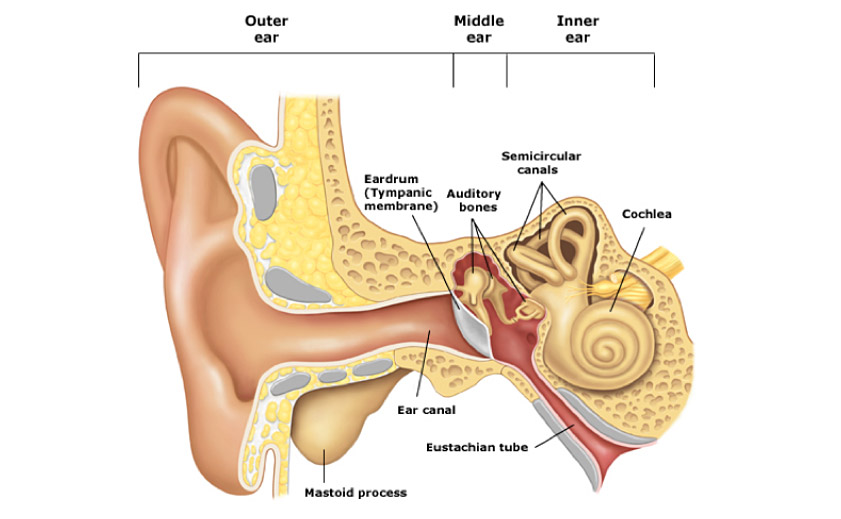
\includegraphics[width=1\textwidth]{anatomy-of-ear.jpg}
		\caption{The figure shows the outer ear, the middle ear and the inner ear.}
		\label{fig:hearing_system}
\end{figure}

\subsection{Functions for ear parts}
The pinna of the outer ear is shaped differently for every person and is very important for localisation of sound event. The shape of the pinna makes amplification, peaks and dips in the sound wave and including the ear canal the changing of the sound in the outer ear is called the \gls{hrtf}. Since the pinna is different for every person, every person have there own \gls{hrtf} and the brain have learned from birth the exact \gls{hrtf}. By changing the \gls{hrtf} on a person, the brain will be confused, but with time the brain can learn a new \gls{hrtf} if necessary. After the sound waves have entered the outer ear and changed by the pinna and the ear canal the tympanic membrane, also called the eardrum, is moving accordingly to the air pressure variation in the ear canal and transmitted to the middle ear.  

The middle ear consist of the three auditory bones, the hammer (malleus), the anvil (incus) and the stirrup (stapes), where the sound wave is travelling mechanically. The bone act as a impedance adaptation from air to liquid and have an amplification of approximation 20 times. The Eustachian tube function is to equalise the air pressure on both side on the eardrum. A build up pressure in the middle ear will affect the hearing negatively. The bone Mallus is attached to the oval window where stapes is attached to the tympanic membrane.

Vibration of the oval window cause wave travelling in the cochlea fluids, those fluid borne wave makes the basilar membrane to vibrate because pressure difference between the cochlear perilymphatic \citep{ho_2017}. The vibration of the basilar membrane gets the inner hair cell to move and generate electric response signal that is transmitted through the auditory nerve to the brain.



\section{Bone conduction of sound}
At the moment there is not a general delimited definiton of what \gls{bc} means, but it is mostly accepted as the sound transmission through the bones of the skull. However, \gls{bc} is not only limited to bones, since it usually also involves transmission through soft tissue and cartilage. Therefore, it can be identified as the transmission of sound energy through the body (bones, soft tissue and cartilage). 
\gls{bc}, although being performed in a localised way, involves the outer, middle and inner ear, as well as the bones surrounding the hearing apparatus and both its fluids and cerebrospinal fluid (CSF) \citep{puria_2013}.
 \begin{figure}[H]
	\centering
		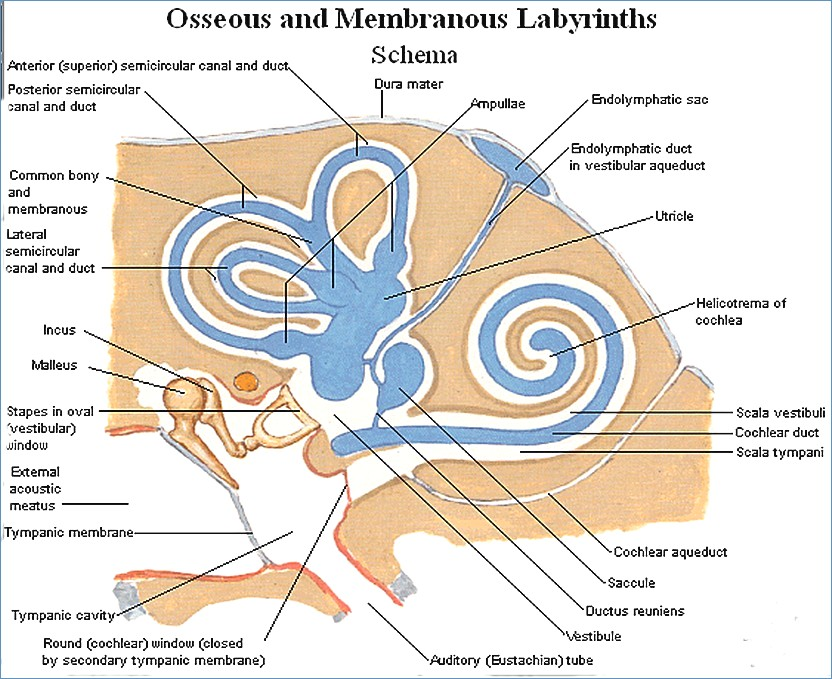
\includegraphics[width=1\textwidth]{more-on-the-vestibular-system-of-anatomy-of-cochlear-aqueduct.jpg}
		\caption{The figure shows the outer ear, the middle ear and the inner ear in detail}
		\label{fig:hearing_system_detail}
\end{figure}
Stenfelt's section 6.1.1 of \citep{puria_2013},starts with the following quote: \enquote{One of the quintessential questions about BC hearing is the end organ for
transforming BC vibration in the skull to neural code}. From this quote, we can infere that the determination of the endpoint for \gls{bc} is not an easy task, and could be the pinnacle in fully understanding \gls{bc} sound transmission.

As explained throughout the referenced section, several studies and experiments have been conducted over the years, leading to the result of identifying the cochlea as such organ. Once the endpoint was identified, it was primordial to understand the ways in which the sound is propagating to reach it.
\subsection{Propagation factors}

When analysing \gls{bc} propagation, we have to take into account three main factors:

\begin{itemize}
\item \textbf{Frequency}: there have been several studies and experiments over time both focused and skull and cochlea vibration patterns. These studies have served as ground for identifying four main modes within the human skull vibration pattern for frequencies below \SI{10}{\kilo\hertz}.
\begin{enumerate}
\item Below \SI{400}{\hertz}: within this range the skull moves as a rigid body (Fig \ref{fig:skull_vibration_pattern}a).\citep{stenfelt_2005b}
\item Between \SI{400}{\hertz} and \SI{1}{\kilo\hertz}: within this range the skull's motion can be described as a mass-spring system(Fig \ref{fig:skull_vibration_pattern}b).
\item Between \SI{1}{\kilo\hertz} and \SI{2}{\kilo\hertz}: at \SI{1}{\kilo\hertz}, the first free resonance of the skull appears \citep{hakansson_1994} and the motion transitions from mass-spring system to a system dominated by wave transmission.
\item Above \SI{2}{\kilo\hertz}: when reaching this range, wave transmission dominates the skull vibration pattern completely, with differences between the cranial vault and the skull base (Fig \ref{fig:skull_vibration_pattern}c).
\end{enumerate}
\begin{figure}[H]
	\centering
		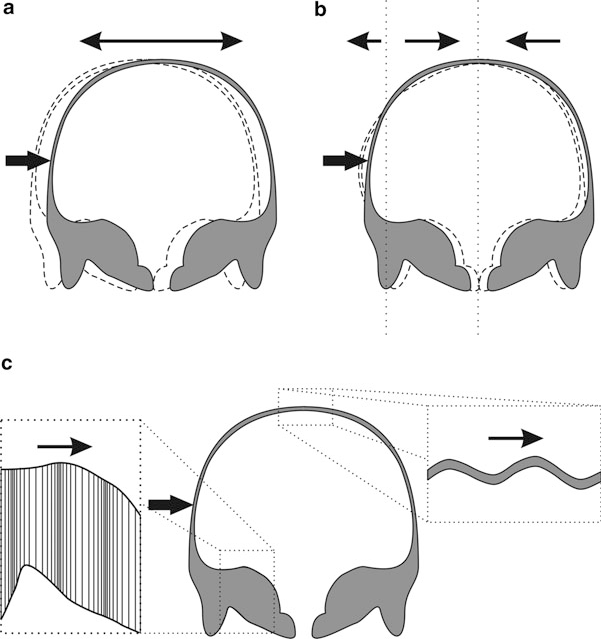
\includegraphics[width=1\textwidth]{skull_vibration_pattern.pdf}
		\caption{Two-dimensional illustration of the vibration modes of the human skull at frequencies between 0.1 and 10 kHz. The thick arrows indicate the stimulation position and the thin arrows indicate the response directions. The rigid body response at the lowest frequencies is illustrated in (a) while the response at frequencies between approximately 0.3–1.0 kHz that is similar to a massspring system is shown in (b) where three sections of the skull move sequentially in opposite directions. In (c) the vibration responses for frequencies above 2 kHz is illustrated differently for the skull base and the cranial vault: at the skull base longitudinal wave propagation dominates the response while a mixture of vibration modes including bending waves is present at the cranial vault \citep{puria_2013}}
		\label{fig:skull_vibration_pattern}
\end{figure}
\item \textbf{Skin} and soft tissue: test
\item \textbf{Position of the transducer}: test
\end{itemize}
\subsection{Influence of Inner/Middle/Outer ear}

Early theories suggested that there were just a couple of pathways dominating the \gls{bc} perception. However, more recent studies suggest that there are five reported pathways for sound vibration to propagate or transmit to the cochlea \citep{zhang_2016}:
\begin{enumerate}
\item External auditory canal sound radiation (outer ear).
\item Inertia of the ossicular chain (middle ear).
\item Inertia of the cochlear fluid (inner ear).
\item Cochlear walls' compression (inner ear).
\item CSF pressure (inner ear).
\end{enumerate}

These pathways can work independently, but all of them add up to the quality of the signal received by the cochlea, and a failure in one of the pathways leads to a decrease in the quality of the received stimuli. In figure \ref{fig:hearing_system_pathway}, this correlation between \gls{bc} and \gls{ac} stimuli is depicted, clearly showing how \gls{bc} stimulation can generate \gls{ac}-like responses in the outer, middle and inner ear.

 \begin{figure}[H]
	\centering
		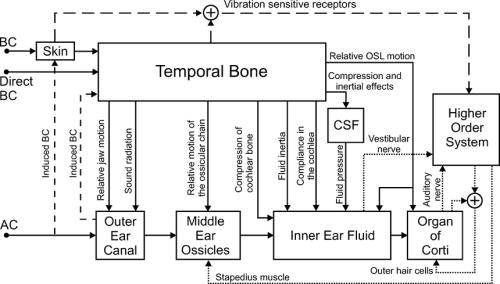
\includegraphics[width=1\textwidth]{ovidweb}
		\caption{The figure shows the transmission path for \gls{bc} \citep{stenfelt_2005}}
		\label{fig:hearing_system_pathway}
\end{figure}



\section{Existing bone conductor}
This section will analyse the most common bone conductors there is used on the marked today. 

\subsection{B71}

\subsection{B81}

\subsection{BEST}

https://pdfs.semanticscholar.org/9407/bf610cf2fc32835a5ca07dcce3d4b4b08599.pdf?_ga=2.147405172.291536821.1537166972-1605440078.1536836079



%%
\part{Design and Optimization}\label{pt:design} 
\graphicspath{{figures/design/}}	
\chapter{Determining \gls{sp}-Parameters}\label{ch:optimization}


%%
\part{Test and Discussion}\label{pt:test}
\graphicspath{{figures/tests/}}
\chapter{Measurement Preparation}


 
%%
\part{Conclusion}\label{pt:conclusion}



\glsresetall
\appendix % Start of appendix
\addtocontents{toc}{\protect\setcounter{tocdepth}{0}} 
%\input{chapters/appendices/_appendices} % Include appendices
%Appendix:

 \graphicspath{{figures/appendix/}}
\part{Appendix}\label{pt:appendix}

 % Include chapters

% For use if report is split up in parts
\bookmarksetup{startatroot}% Goto root of Table of Contents
\addtocontents{toc}{\bigskip}% Add space before next item in Table of Contents

% Appearance of the bibliography
\iflanguage{english}{%
\bibliographystyle{setup/plainnat_en}%
}{%
\bibliographystyle{setup/plainnat_dk}%
}



\bibliography{bib/conference,bib/datasheets,bib/mastersthesis,bib/newsarticles,bib/phdthesis,bib/sciencearticles,bib/standards,bib/techreports,bib/websites,bib/books}
\label{bib:mybiblio}



%\setlength{\chapnumb}{2cm} % Ændrer længden på stregen under kapiteloverskriften så den passer til bilag


\end{document}
